\documentclass[10pt]{article}
\usepackage[letterpaper]{geometry}
\usepackage{listings}
\usepackage{graphicx}
\renewcommand{\figurename}{Imagen}


\title{\textbf{Reporte: Hilos Contra Procesos}}
\author{Diego Ruiz Mora | 2202000335}
\date{29-Septiembre-2023}

\begin{document}
	
	\maketitle
	\section{Funciones generalizadas para los procesos}
	Comenzaremos dando las funciones que nos permitan hacer operaciones en común dentro de los tres programas principales. Solamente necesitamos una función que nos permita obtener la hora, por otro lado una función que nos permita escribir dentro de un archivo, y una sencilla estructura para recuperar la hora. 
	\\\\
	Por comodidad observaremos la estructura, donde tenemos tres enteros que representaran las horas, minutos y segundos: 
	\begin{figure}[h!]
		\centering
		
\includegraphics[width=\linewidth]{estructura.png}
		\caption{Estructura Para Recuperar el Tiempo}
		\label{fig:estructura}
	\end{figure}
	Esto nos permitirá obtener la función que calcula la hora completa, con minutos y segundos. Esta función no recibe nada y regresa como valor un \textit{struct CompleteTime} como el que definimos momentos antes.
	En esta función veremos que tenemos que crear elementos del tipo \textit{time\_t} y otro apuntador a un dato \textit{tm} ambos está contenidos dentro de la librería \emph{time.h} . Seguido a ello, con el uso de la función \textbf{time} y la función \textbf{localtim()} ambas reciben un la referencia del elemento \textit{currentTime}, de esta manera regresamos los valores asignándolos a un elemento del tipo de regreso de la función. 
	\begin{figure}[h!]
		\centering
		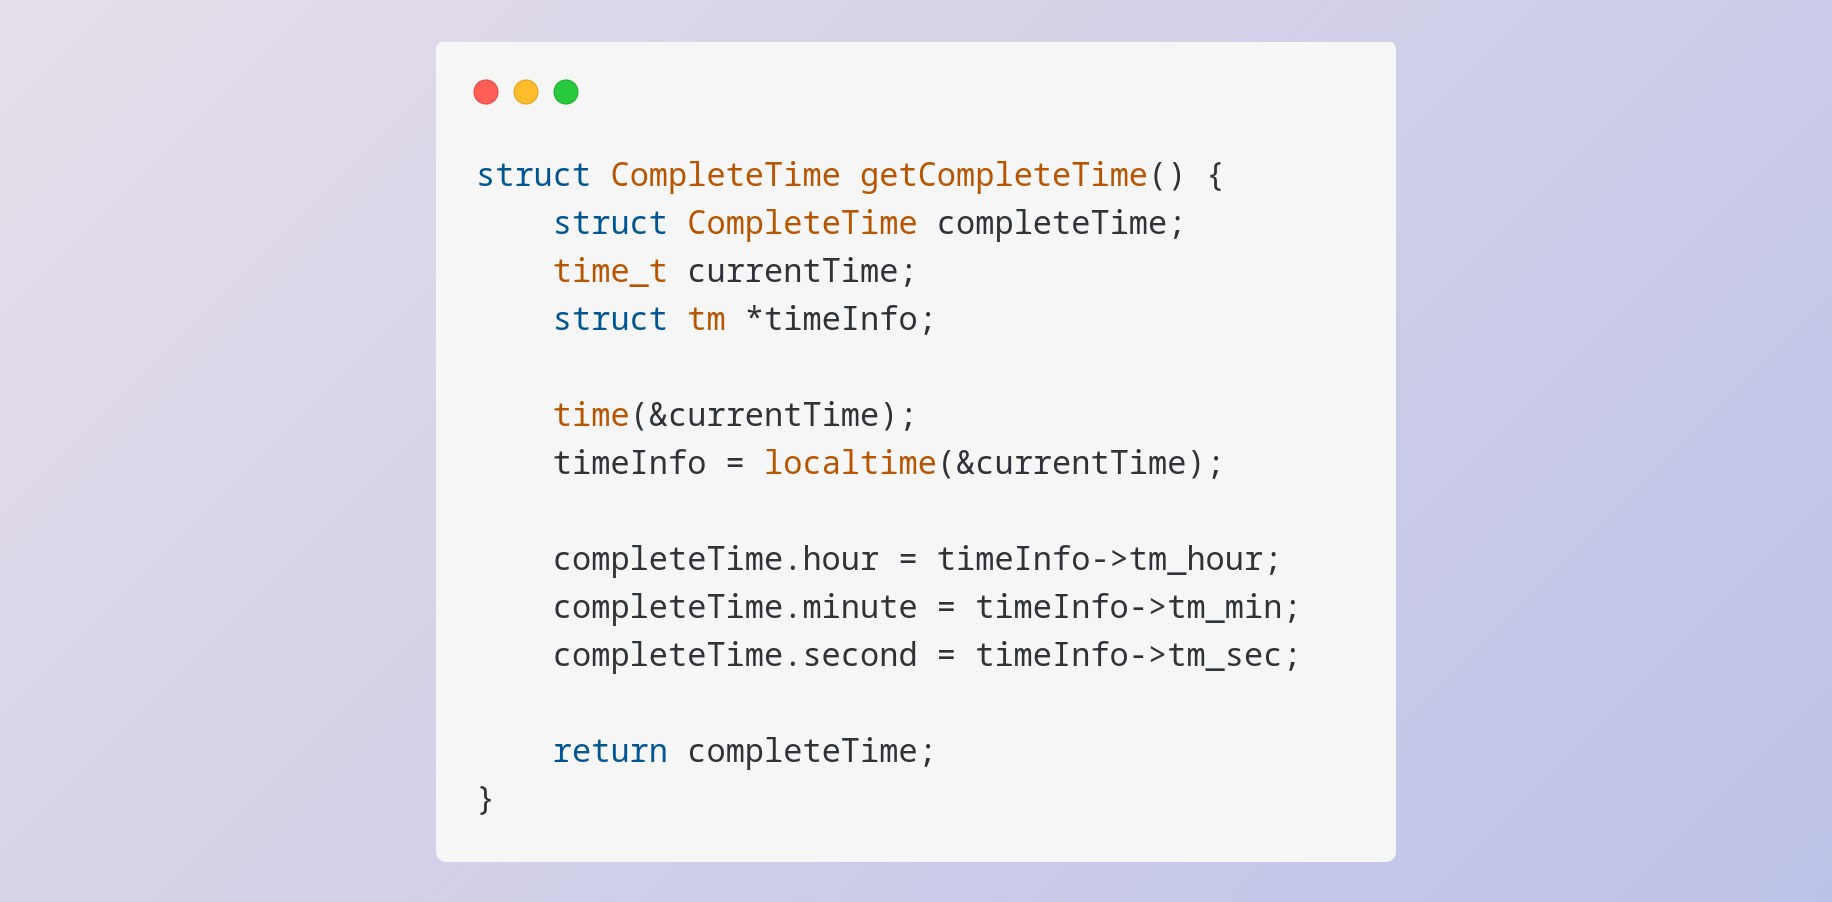
\includegraphics[width=\linewidth]{tiempo.png}
		\caption{Función Para Recuperar el Tiempo}
		\label{fig:tiempo}
	\end{figure}
	\newpage
	Por último veremos la función que nos permite escribir en un archivo, donde tendremos como parámetros dos apuntadores a un elemento del tipo \textbf{char *} que justamente nos indica la posición de inicio de dos cadenas ; el nombre del archivo y la cadena que queremos escribir dentro del archivo.
	\\\\
	Creamos un apuntador del tipo \textit{FILE} que nos permitirá recorrer las posiciones dentro del archivo, inicializandolo con la función \textbf{fopen()} determinar el nombre del archivo y la forma en la que abriremos este archivo. 
	En caso de que este apuntador sea distinto de \textbf{NULL} nos permitirá escribir en el, con la función \textbf{fprintf()} y cerraremos la cadena de escritura con la función \textbf{fclose()}.
	\begin{figure}[h!]
		\centering
		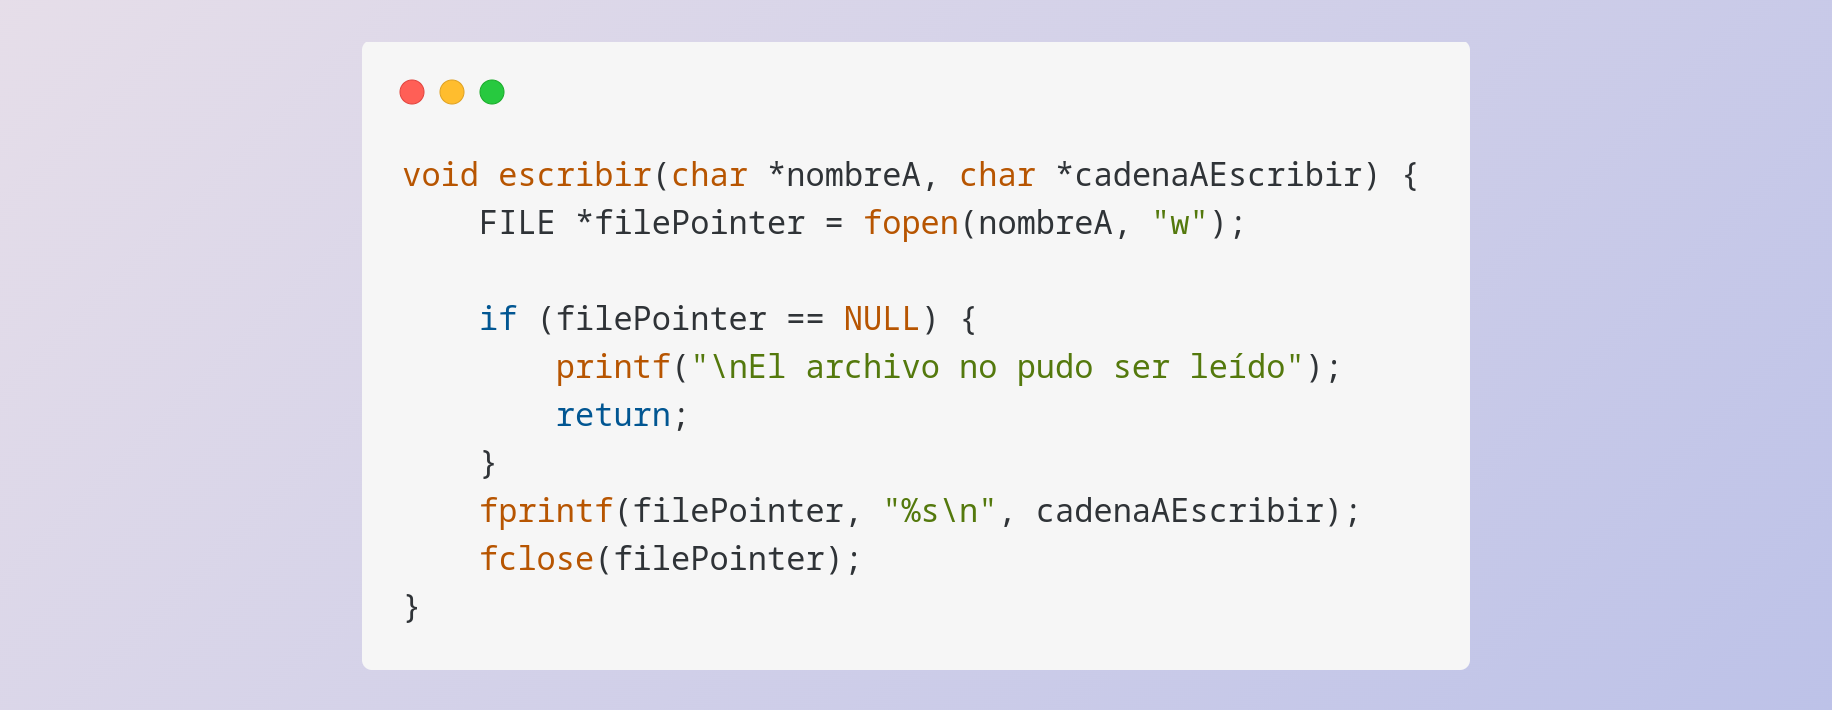
\includegraphics[width=\linewidth]{escritura.png}
		\caption{Función Para Escribir En Un Archivo}
		\label{fig:escritura}
	\end{figure}
	
	\section{Programa de creación de procesos}
	\begin{figure}[h!]
		\centering
		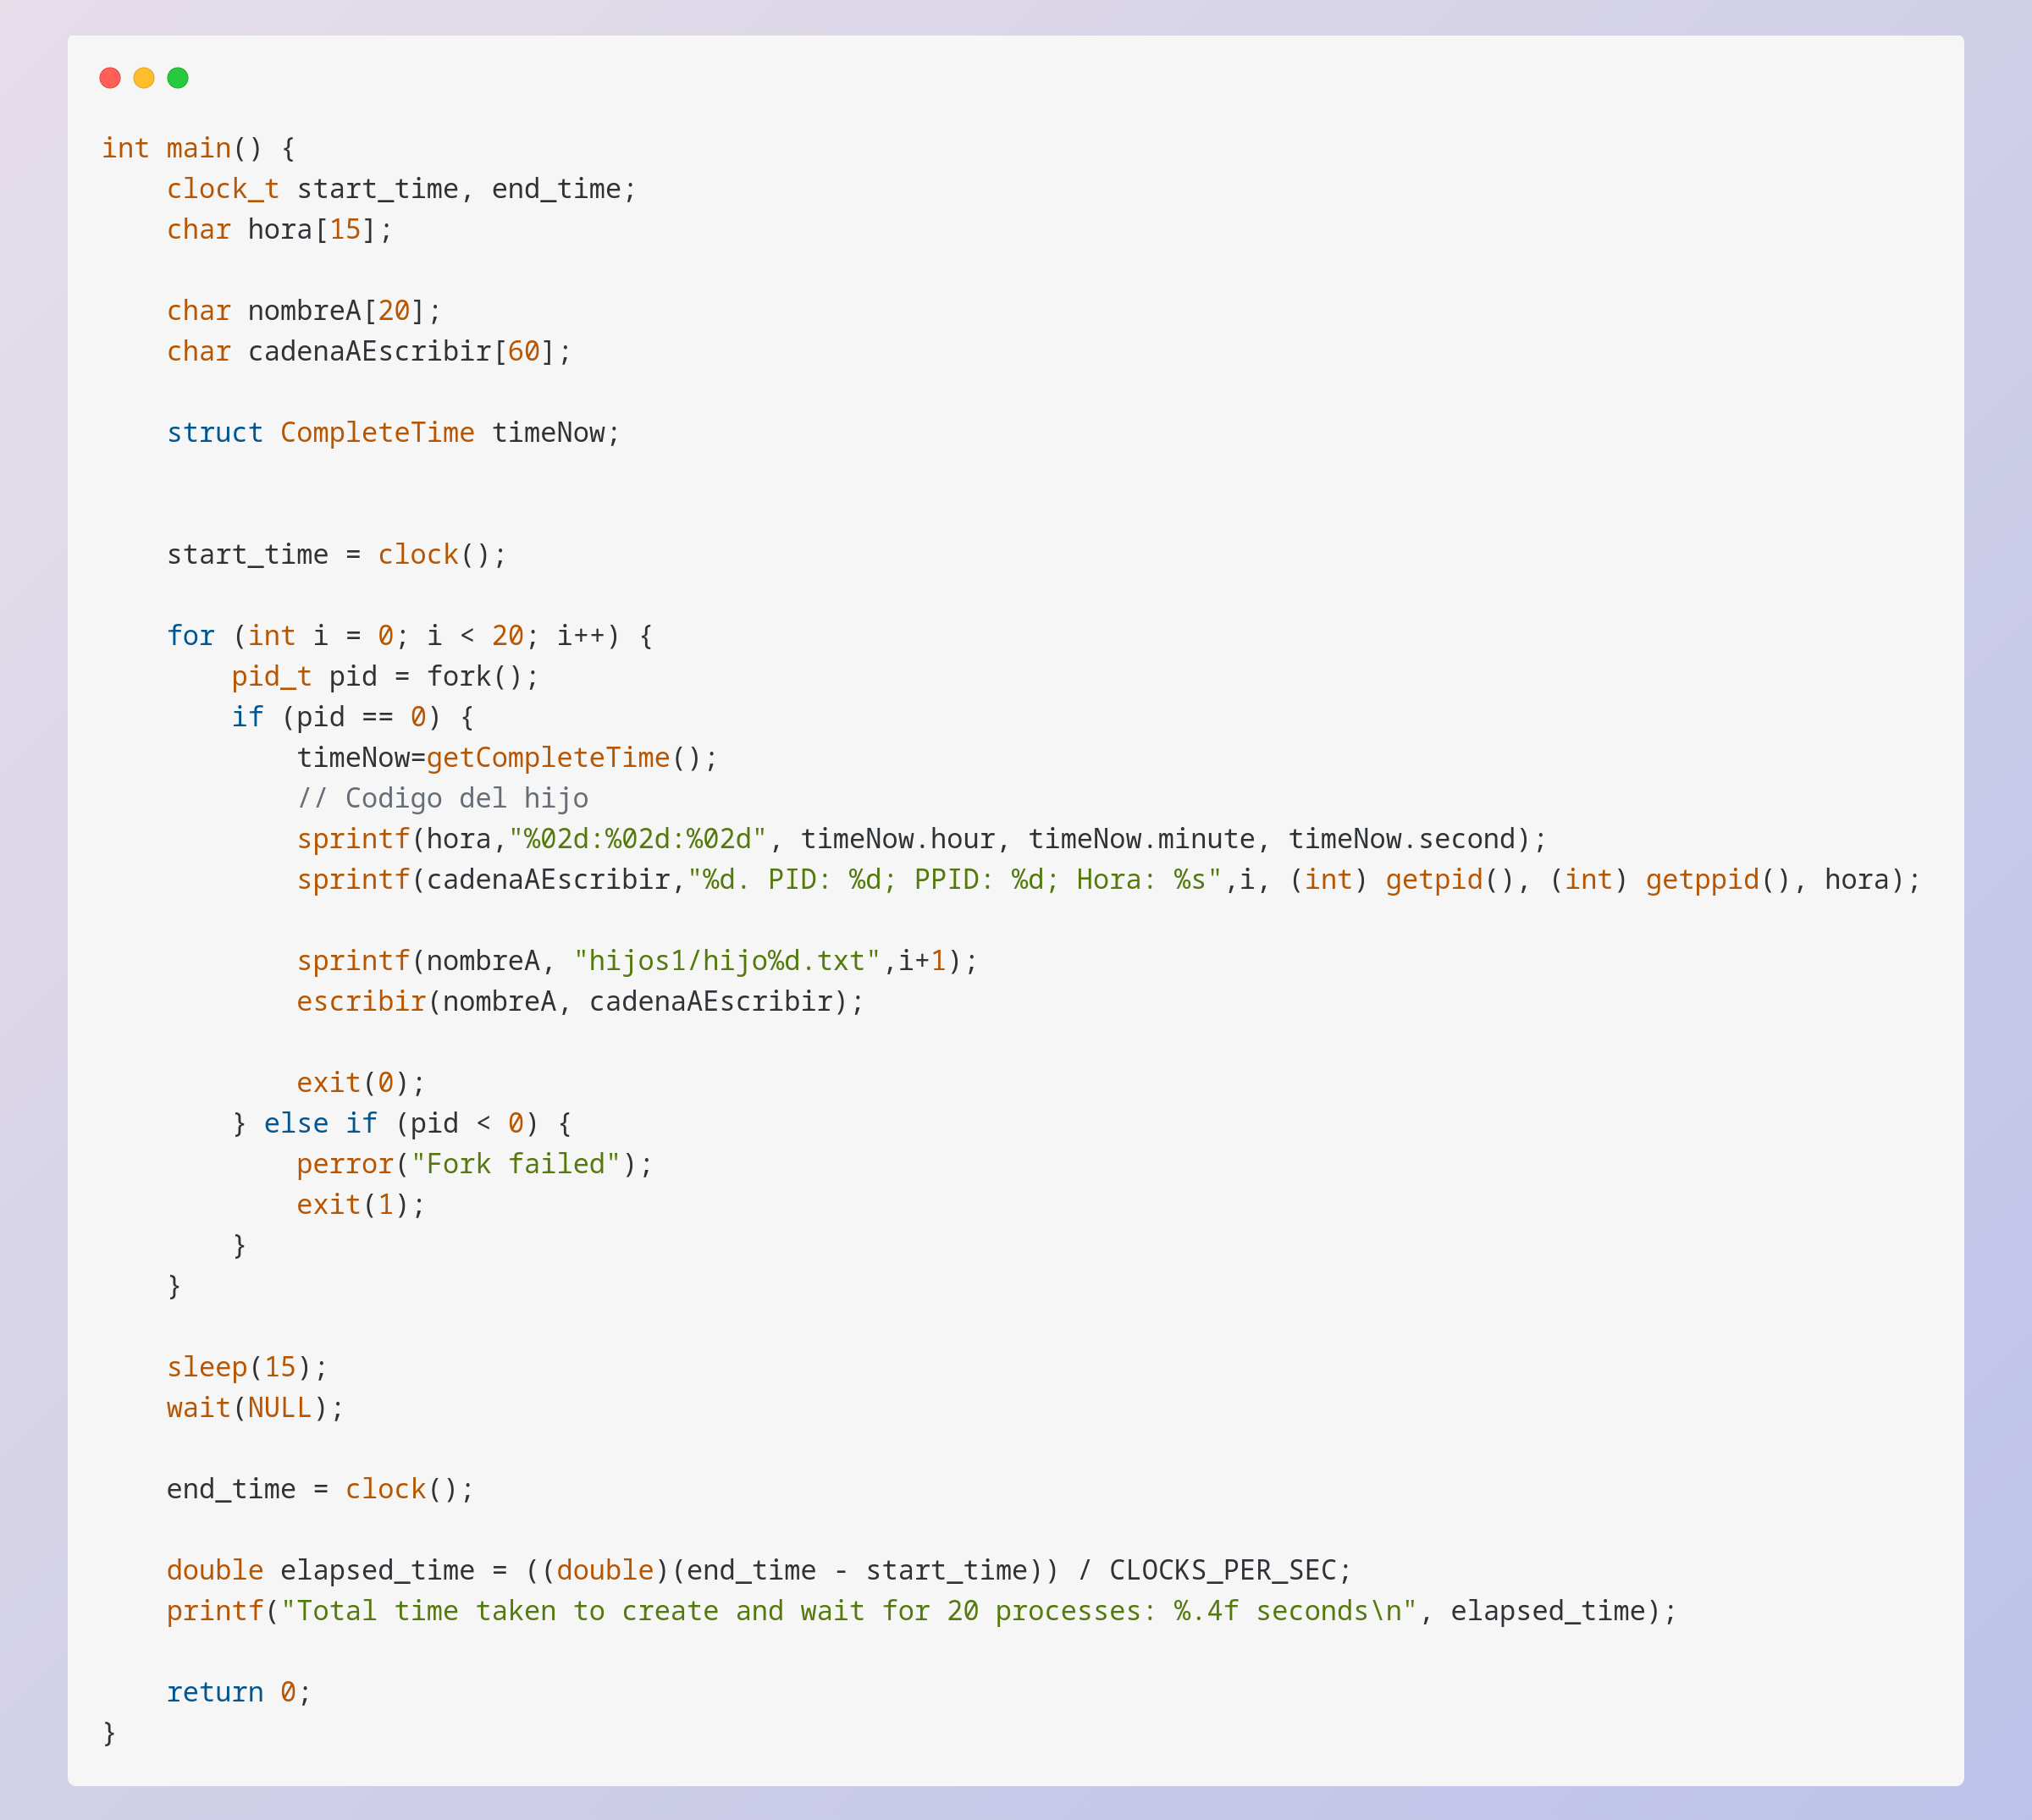
\includegraphics[width=\linewidth]{pvh1.png}
		\caption{Programa Para Crear 20 Procesos}
		\label{fig:pvh1}
	\end{figure}
	Notaremos que la función tiene bastante puntos a destacar. Primero que nada tendremos que crear unos datos del tipo \textit{clock\_t} que nos permitirá obtener el punto de inicio y de termino de programa para poder desplegar el tiempo empleado en la creación de los veinte procesos. Así mismo un arreglo de caracteres que nos ayudará a escribir la hora que obtenemos para cada archivo. 
	Luego declararemos otros dos arreglos de carácter para la creación del archivo. Seguido de ello un \textit{struct CompleteTime} que nos permite obtener la hora en un punto exacto. 
	\\\\\\
	Seguido comenzamos un ciclo que se repita veinte veces, dentro de el declaramos una variable del tipo \textit{pid\_t} para poder hacer la llamada a sistema \textbf{fork()} para duplicar el proceso, lo cual ocurre justo después. Esto nos permite diferenciar entre el proceso hijo el proceso padre. En caso de ser uno de los hijos deberemos primero que nada tomar el tiempo en ese momento y escribirla en la cadena de la hora. 
	\\\\
	Luego tendremos que escribir en la cadena que pasaremos al archivo. La cual contiene el identificador del proceso, el identificador del proceso padre  y la hora a la que fue creado este hijo. Después de ello escribimos en la cadena que será el nombre del archivo, que es justo la siguiente instrucción mandando a llamar a la función que escribe. Terminamos esta parte con una salida exitosa. 
	\\\\
	Luego haremos una pequeña pausa, que se puede omitir, solamente la utilizamos para lograr visualizar en las herramientas los 20 procesos que se crearon. Que es algo parecida a la idea de la llamada de sistema \textbf{wait(NULL)} para esperar a los procesos hijos a que concluyan. 
	\\\\
	Marcamos el tiempo de finalización de la creación y terminación de procesos para poco después hacer la diferencia, el cociente con un tipo de datos para obtener el dato en segundos y \emph{castearla} a un \textit{double} para visualizarlo mediante una impresión. 
	\section{Programa de creación de hilos}
	\subsection{Función imagen para los hilos creados}
	\begin{figure}[h!]
		\centering
		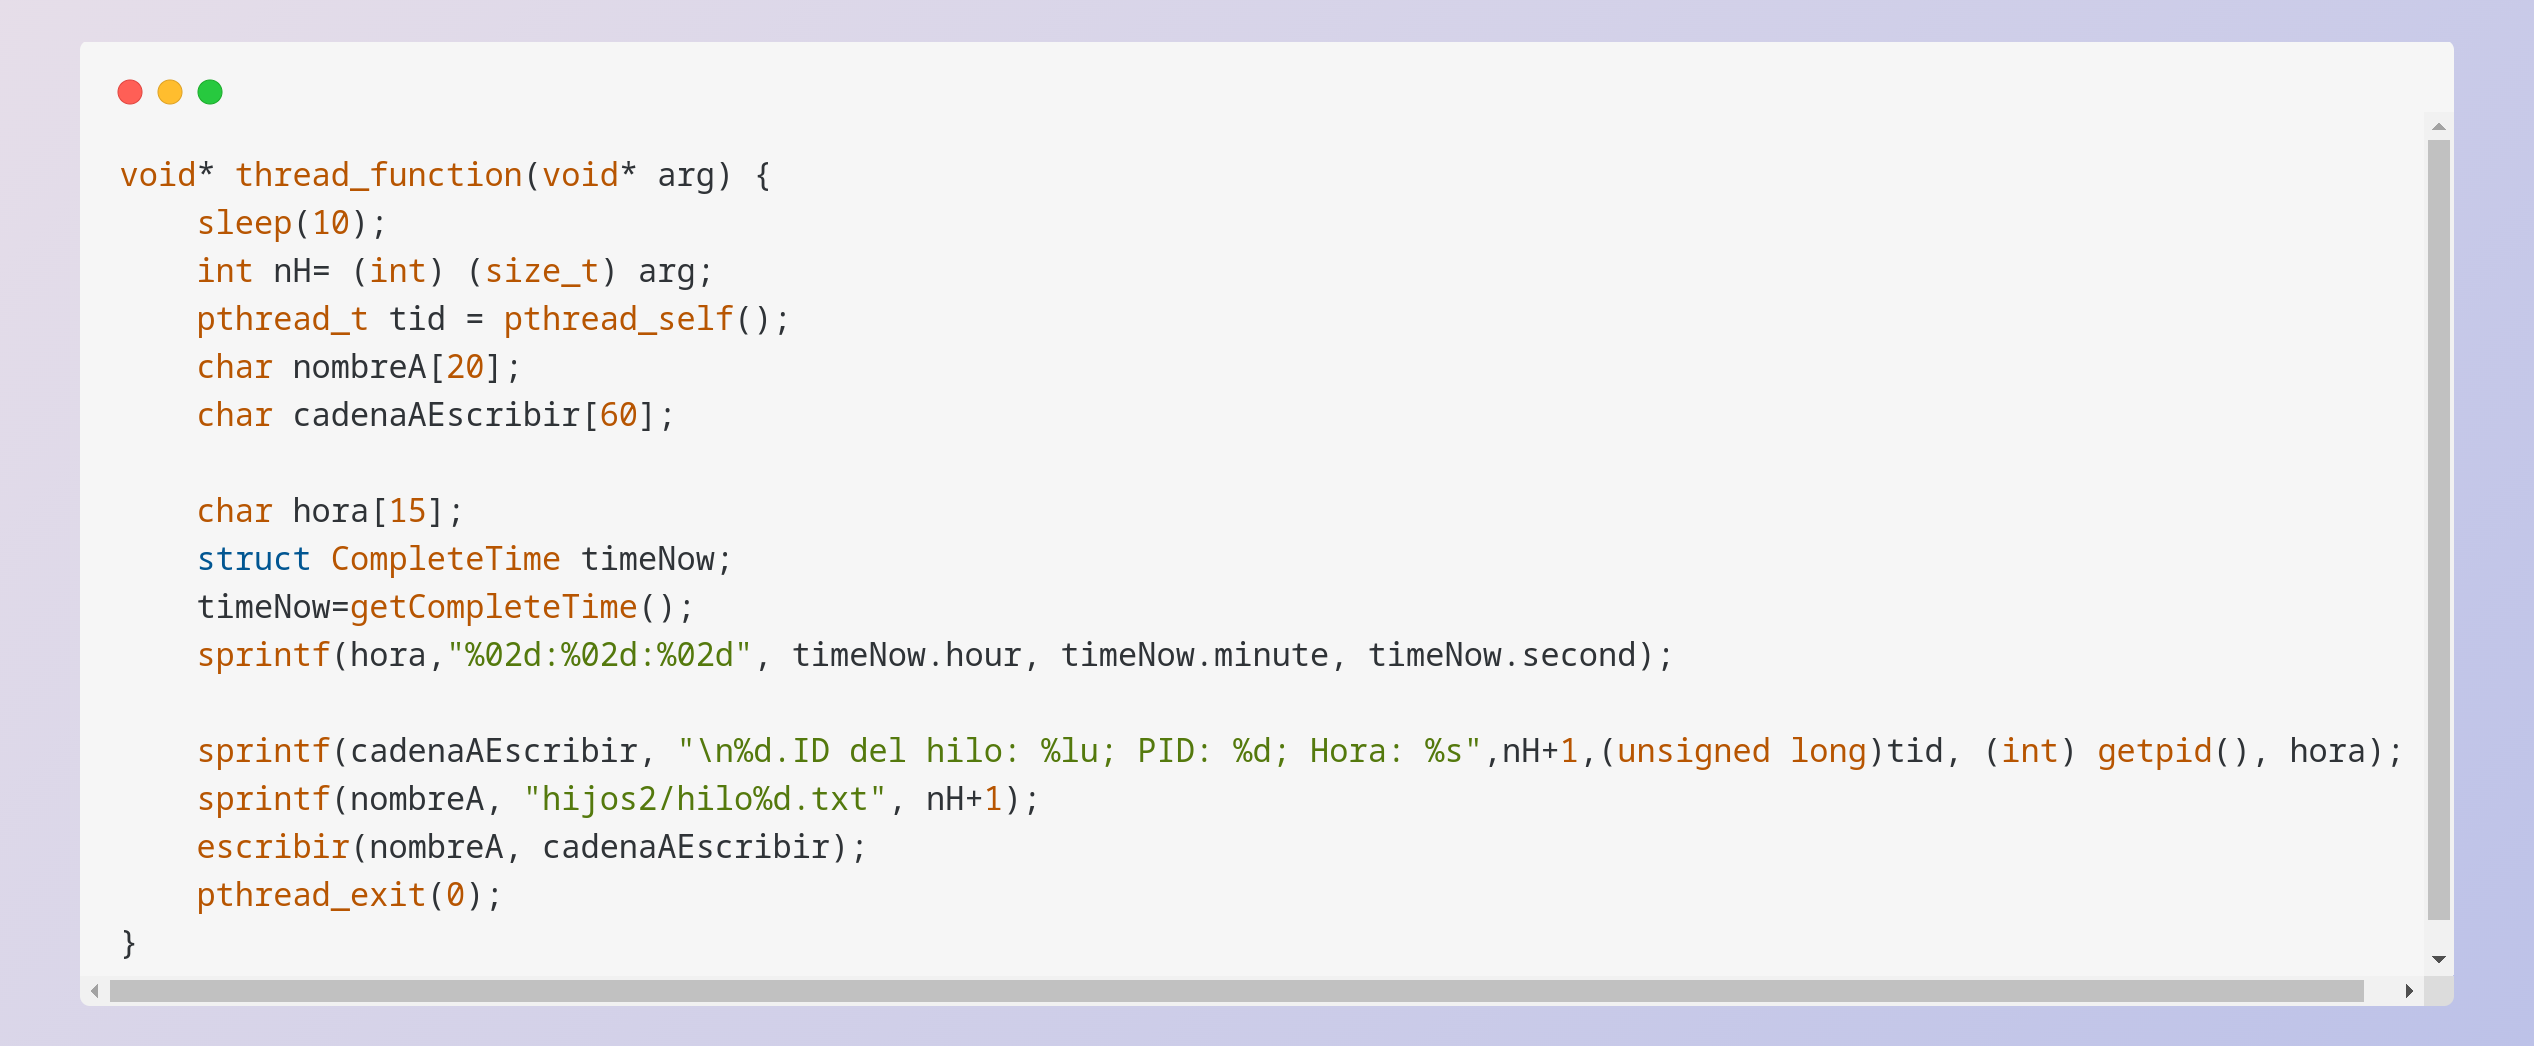
\includegraphics[width=\linewidth]{funH.png}
		\caption{Función Imagen Para Los Hilos}
		\label{fig:funH}
	\end{figure}
	Como bien sabemos tenemos que crear una función que reciba un apuntador a nulo y que regrese un apuntador a nulo, que es justamente el caso que tenemos con esta función. Empezamos con una llamada a sistema \textbf{sleep()} que puede ir o no y que tiene la intención de visualizar los hilos con distintas herramientas. 
	\\\\
	Luego obtendremos los parámetros que en este caso será solamente el número de hilo que se creó, también tenemos que declarar un elemento del tipo \textit{pthread\_t} inicializandolo con el valor del identificador del hilo. Además dos cadenas, ambas para escribir en la cadena, tal como lo vimos en el caso pasado y por ultimo un arreglo de caracteres para la hora.
	\\\\
	De hecho podemos notar que el proceso para encontrar la hora en el momento exacto es lo mismo, por tal razón omitiremos la expliación del mismo. Después escribiremos en la cadenas para la generación del archivo y por ultimo \textbf{pthread\_exit(0)} para informar que el hilo termina de manera correcta. 
	\subsection{Función principal para la creación de hilos}
	\begin{figure}[h!]
		\centering
		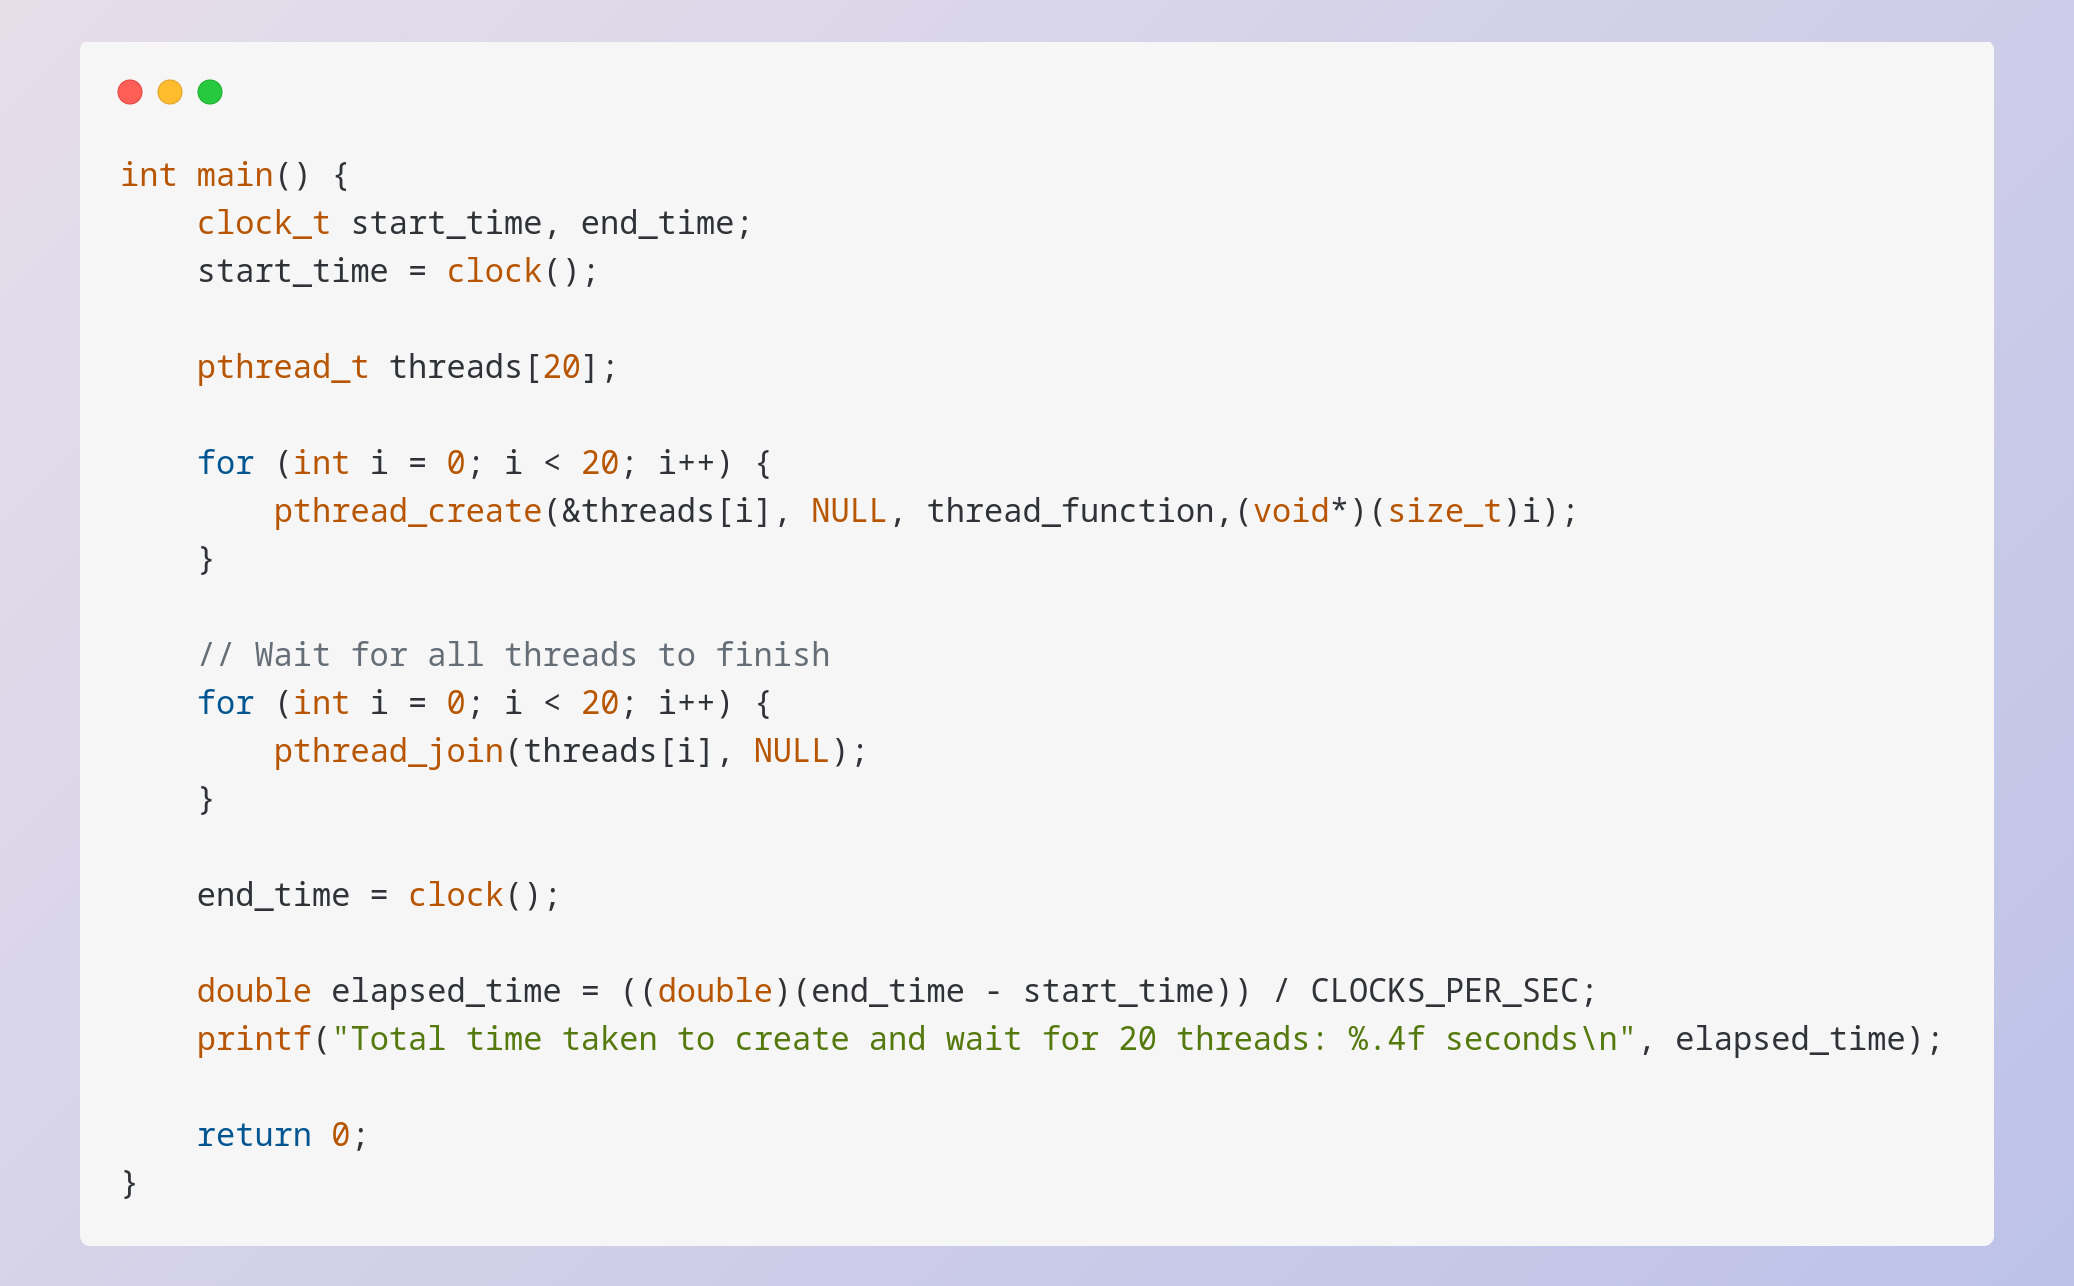
\includegraphics[width=\linewidth]{pvh2.png}
		\caption{Programa Para Crear 20 Hilos}
		\label{fig:pvh2}
	\end{figure}
	Notaremos que al igual que en el caso pasado tenemos dos elementos que nos permitirán obtener el inicio y fin de la creación. De hecho, comenzamos con eso,  inicializando  la variable que nos marca el comienzo de la creación de hilos. Luego declaremos un arreglo de elmentos del tipo \textit{pthread\_t} que nos permite diferenciar a cada uno de los hilos. 
	\\\\
	Para la creación de los 20 hilos usaremos un ciclo y dentro de el la instrucción \textbf{pthread\_create()} con argumentos la referencia al arreglo de identificadores de hilos, \textit{NULL} para el caso de la estructura que inicializa los hilos; osea la que es por defecto, la función que le da imagen al hilo y por ultimo los argumentos que recibirá el hilo, que como bien se menciono será el numero de hilo creado. 
	\\\\
	Mas abajo haremos uso de otro ciclo para repetir la instrucción \textbf{pthread\_join} que nos permite esperar a que los hilos se terminan de ejecutar. Esta función recibe el identificador de hilo y un \textit{NULL} que son los valores que recuperaremos al termino del hilo. Terminamos justamente con lo mismo que en el caso pasado, el cálculo y la impresión del total de tiempo de ejecución. 
		
\end{document}